\section{Algoritmo optimizado da ImageBlur}
\label{sec:imageblur/optimal}

\subsection{Imagem Integral}

Considerando $img$ como uma matriz $m \times n$, onde $m~=~img\rightarrow height$ e $n~=~img\rightarrow width$, vamos gerar uma matriz $m+1 \times n+1$ onde a primeira linha e a primeira coluna vão ser zeros, a partir daí, o elemento $(y,x)$ desta matriz irá corresponder ao elemento $(y-1,x-1)$ da matriz da imagem com $x\in[1,n]$ e $y\in[1,m]$. Esta nova imagem será armazenada como um array de $m+1~*~n+1$ elementos, com 32 bits cada (visto que será um array de inteiros).

Para inicializar a matriz, usamos as linhas de código:

\begin{lstlisting}[language=C]
    int integral_width = img->width + 1;
    int integral_height = img->height + 1;
    int* integral = (int*)calloc(integral_width * integral_height, sizeof(int));
\end{lstlisting}

Agora vamos ter de completar o resto das células. Cada célula da nova matriz será igual à soma de todos os pixeis que estão acima e à esquerda do mesmo.

\begin{figure}[H]
    \centering
    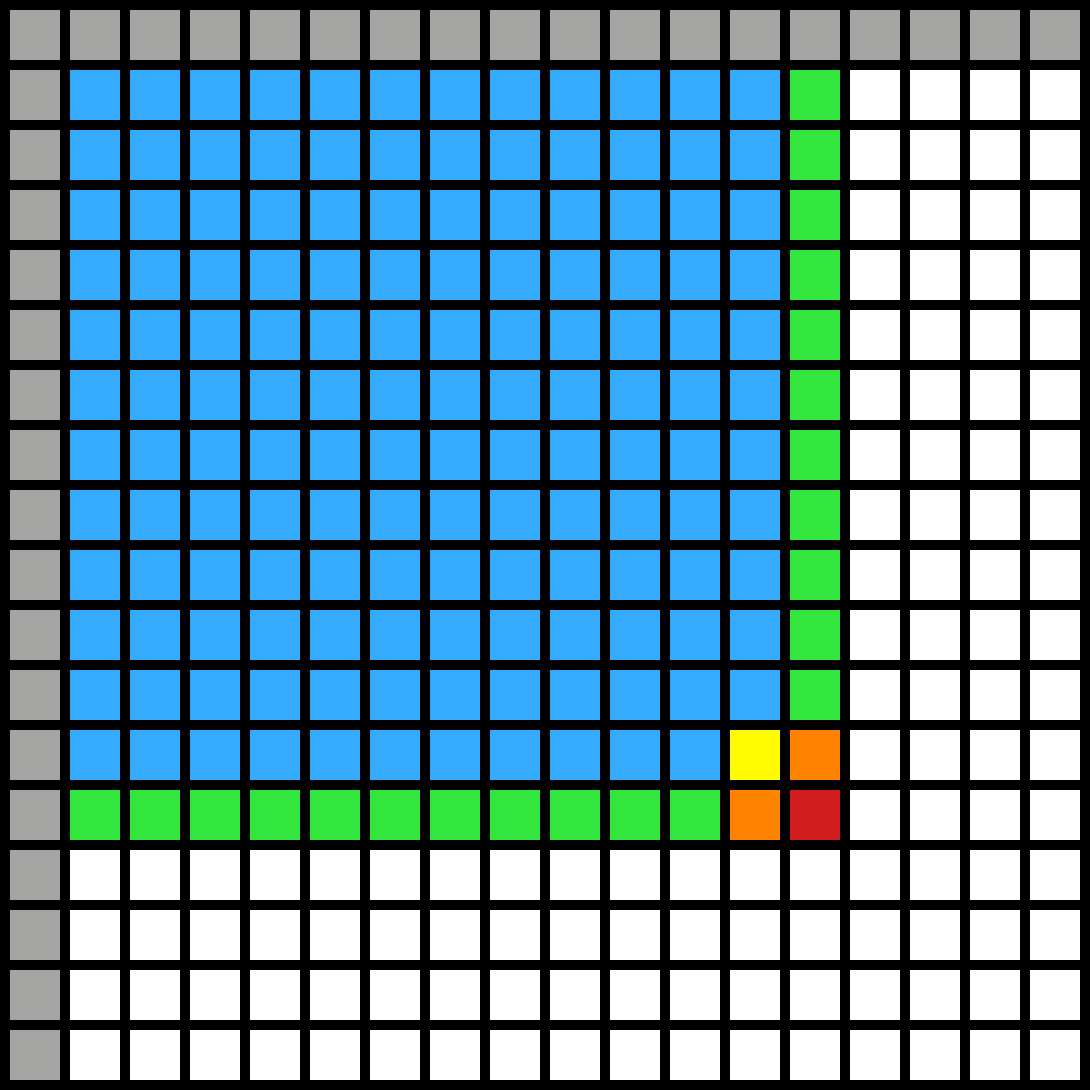
\includegraphics[width=0.4\linewidth]{images/integral-matrix.png}
    \caption{Representação da matriz integral}
\end{figure}

Como podemos ver na figura acima, para calcular o pixel representado a \textcolor{red}{\textbf{vermelho}} ($I_{(y,x)}$), teremos de adicionar ao pixel original da imagem, depois, o elemento representado acima a \textcolor{orange}{\textbf{laranja}} ($I_{(y-1,x)}$) que já contém todos os pixeis acima e à esquerda do mesmo (representados a \textcolor{green}{\textbf{verde}} acima do pixel mencionado), e por fim, teremos de adicionar o elemento representado à esquerda também a \textcolor{orange}{\textbf{laranja}} ($I_{(y, x-1)}$) que contém todos os pixeis na linha horizontal à esquerda do mesmo (representados a \textcolor{green}{\textbf{verde}} à esquerda do pixel mencionado). Uma vez que o pixel $I_{(y,x-1)}$, também contém a área acima dele (parte já incluída pelo pixel $I_{(y-1,x)}$), então teremos de remover a parte duplicada (área representada a \textcolor{blue}{\textbf{azul}}) que corresponde ao valor do pixel representado a \textcolor{yellow}{\textbf{amarelo}} ($I_{(y-1,x-1)}$). Com isto, podemos concluir que a expressão para cálcular a área a atribuir a um determinado pixel será:

\begin{equation}
    I_{(y,x)} = O_{(y-1,x-1)} + I_{(y-1,x)} + I_{(y,x-1)} - I_{(y-1,x-1)}
\end{equation}\label{eq:equacao-para-integral}

De notar que as células representadas a \textcolor{gray}{\textbf{cinzento}} serão as células cujo valor do elemento será sempre zero.

Para calcular todas estas células da matriz, usamos as linhas de código:

\begin{lstlisting}[language=C]
    for (int y = 1; y < integral_height; y++) {
        for (int x = 1; x < integral_width; x++) {
            integral[y * integral_width + x] = ImageGetPixel(img, x - 1, y - 1)   
                + integral[(y - 1) * integral_width + x]                          
                + integral[y * integral_width + (x - 1)]                          
                - integral[(y - 1) * integral_width + (x - 1)];                   
        }
    }
\end{lstlisting}

\pagebreak

\subsection{Imagem desfocada}

Uma vez que já temos a imagem integral, podemos agora calcular a imagem desfocada. Para isso, vamos percorrer a imagem integral e para cada pixel, teremos de efetuar o seguinte procedimento:

\begin{enumerate}

\item {
\textbf{Calcular os cantos do retângulo de blur}

Vamos calcular a soma dos pixeis que estão dentro do retângulo de dimensões $2dx+1$ e $2dy+1$ para o comprimento e largura, respetivamente, centrado no pixel atual. Poderemos obter esse retângulo usando o canto superior esquerdo bem como o canto inferior direito.

\begin{enumerate}
    

    \item {
        \textbf{Canto superior esquerdo}

        Para obter cada uma das coordenadas deste ponto, teremos de subtrair a cada coordenada do pixel, os valores do $dy$ e $dx$, $dy$ para a borda superior e $dx$ para a borda da esquerda. No caso do resultado de uma dessas coordenadas ultrapassar um dos limites mínimos do retângulo, então esta coordenada deverá ser o limite mínimo. Este limite normalmente seria 0 mas visto que na imagem integral temos uma linha e uma coluna extra em cima e à esquerda, então temos de somar 1 a esses limites para compensar pelos pixeis extra e redefinir o início da parte útil da matriz. Isto fará que o limite mínimo seja 1 à esquerda e em cima. Para calcular as coordenadas, usamos as linhas de código: 

        \begin{lstlisting}[language=C]
int x1 = x - dx < 1 ? 1 : x - dx;
int y1 = y - dy < 1 ? 1 : y - dy;
        \end{lstlisting}
    }
    \item {
        \textbf{Canto inferior direito}

        Para obter cada uma das coordenadas deste ponto, teremos de somar a cada coordenada do pixel, os valores do $dy$ e $dx$, $dy$ para a borda inferior e $dx$ para a borda da direita. No caso do resultado de uma dessas coordenadas ultrapassar um dos limites máximos do retângulo, então esta coordenada deverá ser o limite máximo. Uma vez que deste lado não temos nenhuma linha ou coluna extra, o limite máximo será o último indice, ou seja, $integral\_width-1$. Isto fará que o limite máximo seja a largura menos 1 à direita e a altura menos 1 em baixo. Aos resultados, teremos de adicionar o valor 1 visto que não é contabilizada a linha/coluna do pixel central. Para calcular as coordenadas, usamos as linhas de código:

        \begin{lstlisting}[language=C]
int x2 = x + dx + 1 > integral_width - 1 ? integral_width - 1 : x + dx + 1;
int y2 = y + dy + 1 > integral_height - 1 ? integral_height - 1 : y + dy + 1;
        \end{lstlisting}
    }
\end{enumerate}
}

\item {
\textbf{Cálculo da quantidade de pixeis}

Para calcular a quantidade de pixeis que estão dentro do retângulo, basta calcular a área do retângulo em pixeis, ou seja, a multiplicação do comprimento pela largura. Para tal, usamos a linha de código:

\begin{lstlisting}[language=C]
    int count = (x2 - x1) * (y2 - y1);
\end{lstlisting}
}

\pagebreak

\item {
\textbf{Cálculo da soma}

\begin{figure}[H]
    \centering
    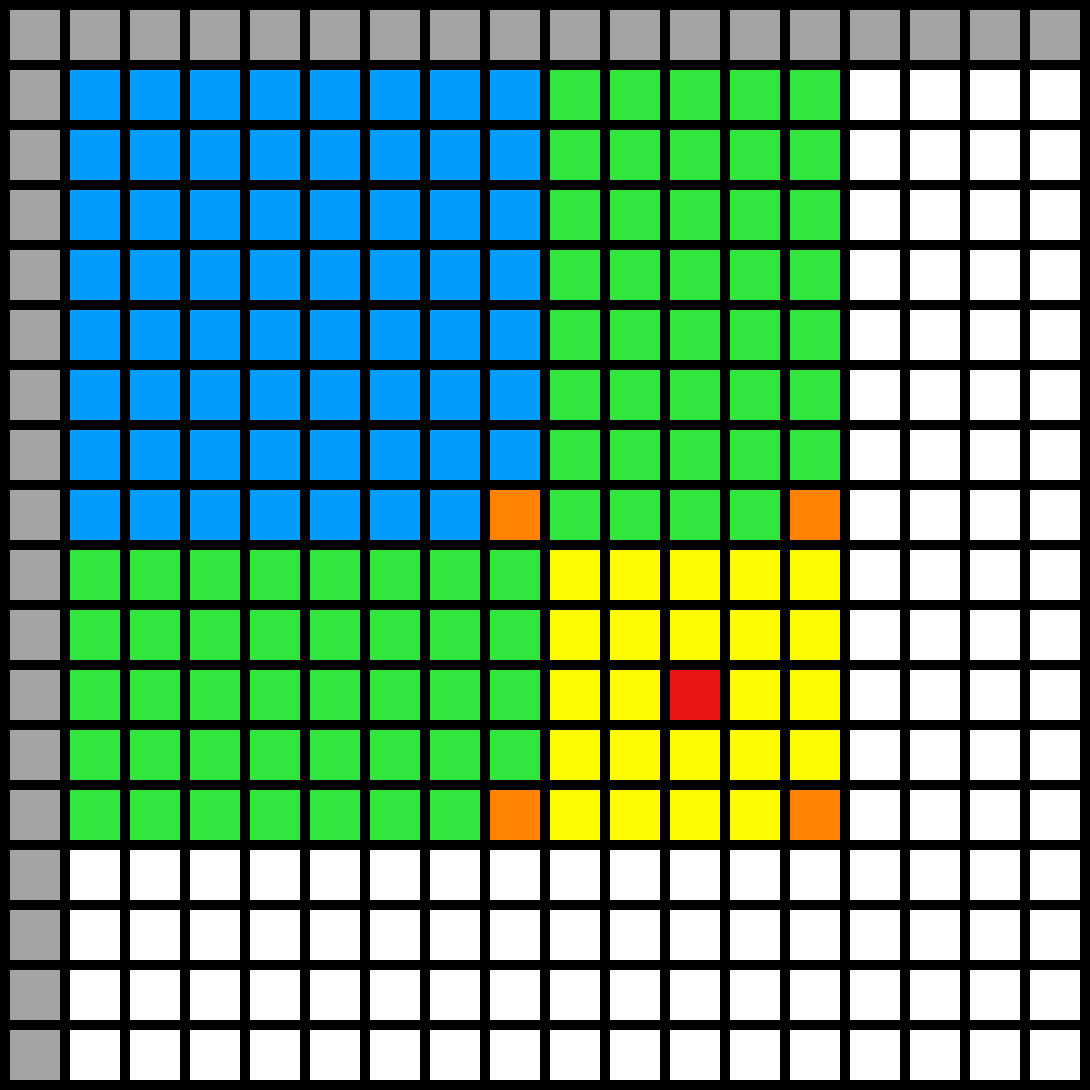
\includegraphics[width=0.4\linewidth]{images/rectangle-area.png}
    \caption{Representação do retângulo de blur}
\end{figure}

Como podemos ver pela figura anterior, para conseguir a área pretendidada (representada a \textcolor{yellow}{\textbf{amarelo}}), temos de usar como base a área associada ao pixel do canto inferior direito e subtrair a área associada ao pixel do canto superior direito (área acima do retângulo) bem como subtrair a área associada ao pixel do canto inferior esquerdo (área à esquerda do retângulo). Estas áreas exteriores ao retângulo estão representadas a \textcolor{green}{\textbf{verde}}. Visto que uma parte destas áreas coincide, temos de tirar a parte duplicada que será a área associada ao pixel do canto superior esquerdo e representada a \textcolor{blue}{\textbf{azul}} na imagem. Importante notar que enquanto que o canto inferior direito será incluído na área, os outros 3 cantos não serão. A partir disto, podemos obter a soma do retângulo de blur a partir da seguinte expressão:

\begin{equation}
    S_{(y,x)} = I_{(y2,x2)} - I_{(y1,x2)} - I_{(y2,x1)} + I_{(y1,x1)}
\end{equation}\label{eq:equacao-para-soma}

Para calcular o resultado desta expressão, usamos as linhas de código:

\begin{lstlisting}[language=C]
    int sum = integral[y2 * integral_width + x2]
            - integral[y1 * integral_width + x2]
            - integral[y2 * integral_width + x1]
            + integral[y1 * integral_width + x1];
\end{lstlisting}
}

\item {
\textbf{Definir o novo valor do pixel}

Para definir o novo valor do pixel, basta dividir a soma pelo número de pixeis que estão dentro do retângulo. Para tal, usamos a linha de código:

\begin{lstlisting}[language=C]
    ImageSetPixel(img, x, y, (sum + count / 2) / count);
\end{lstlisting}

De notar que somamos $count/2$ à soma para que o resultado da divisão seja arredondado corretamente.
}

Após repetir este procedimento para todos os pixeis da imagem, obtemos a imagem desfocada.
\end{enumerate}
